
\documentclass[xcolor=dvipsnames]{beamer}  % for hardcopy add 'trans'

\mode<presentation>
{
  \usetheme{Singapore}
  % or ...
  \setbeamercovered{transparent}
  % or whatever (possibly just delete it)
}

\usefonttheme{professionalfonts}
\usepackage[russian]{babel}
% or whatever
%\usepackage[latin1]{inputenc}
% or whatever
%\usepackage{times}
%\usepackage[T1]{fontenc}
% Or whatever. Note that the encoding and the font should match. If T1
% does not look nice, try deleting the line with the fontenc.

%%%%%%%%%%%%%%%%%%%%%% start my preamble %%%%%%%%%%%%%%%%%%%%%%


\addtobeamertemplate{navigation symbols}{}{%
    \usebeamerfont{footline}%
    \usebeamercolor[fg]{footline}%
    \hspace{1em}%
    \insertframenumber/\inserttotalframenumber
} 

\setbeamercolor{footline}{fg=blue}
\setbeamerfont{footline}{series=\bfseries}


%\usepackage{epsfig}
\usepackage{graphicx}
\graphicspath{{./figs_code/}}

\usepackage{amsmath, amssymb, amsthm}

\usepackage{fancyvrb}

\usepackage{tikz}
\usetikzlibrary{arrows}
\usetikzlibrary{calc}
\usetikzlibrary{intersections}
\usetikzlibrary{decorations}
\usepackage{pgf}
\usepackage{pgfplots}
\pgfplotsset{compat=1.13}

\usepackage{graphviz}
 
\usepackage{verbatim}


\usepackage{algorithmicx,algpseudocode}


%font
\usepackage{mathpazo}
%\usepackage[usenames, dvipsnames]{color}

%\usepackage[linesnumbered, ruled, lined]{algorithm2e}

\usepackage{xr}
\externaldocument[ET-]{et}


\newcommand*{\theorembreak}{\usebeamertemplate{theorem end}\framebreak\usebeamertemplate{theorem begin}}

\newcommand{\newtopic}[1]{\textcolor{Green}{\Large \bf #1}}
\newcommand{\navy}[1]{\textcolor{Blue}{\bf #1}}
\newcommand{\navymth}[1]{\textcolor{Blue}{#1}}
\newcommand{\red}[1]{\textcolor{red}{#1}}


\definecolor{pale}{RGB}{235, 235, 235}
\definecolor{pale2}{RGB}{175,238,238}
\definecolor{turquois4}{RGB}{0,134,139}

% Typesetting code
\definecolor{bg}{rgb}{0.95,0.95,0.95}
\usepackage{minted}
\usemintedstyle{friendly}
\newminted{python}{mathescape,frame=lines,framesep=4mm,bgcolor=bg}
\newminted{ipython}{mathescape,frame=lines,framesep=4mm,bgcolor=bg}
\newminted{julia}{mathescape,frame=lines,framesep=4mm,bgcolor=bg}
\newminted{c}{mathescape,linenos=true}
\newminted{r}{mathescape,  frame=none, baselinestretch=1, framesep=2mm}
\renewcommand{\theFancyVerbLine}{\sffamily
    \textcolor[rgb]{0.5,0.5,1.0}{\scriptsize {\arabic{FancyVerbLine}}}}


\usepackage{stmaryrd}

\newcommand{\Fact}{\textcolor{Brown}{\bf Факт. }}
\newcommand{\Facts}{\textcolor{Brown}{\bf Факты }}
\newcommand{\keya}{\textcolor{turquois4}{\bf Ключевая идея. }}
\newcommand{\Factnodot}{\textcolor{Brown}{\bf Факт }}
\newcommand{\Eg}{\textcolor{ForestGreen}{Пример. }}
\newcommand{\Egs}{\textcolor{ForestGreen}{Примеры. }}
\newcommand{\Ex}{{\bf Ex. }}
\newcommand{\Thm}{\textcolor{Brown}{\bf Теорема. }}
\newcommand{\Prf}{\textcolor{turquois4}{\bf Доказательство. }}
\newcommand{\Ass}{\textcolor{turquois4}{\bf Допущение.}} 
\newcommand{\Lem}{\textcolor{Brown}{\bf Лемма. }}

%source code 



% cali
\usepackage{mathrsfs}
\usepackage{bbm}
\usepackage{subfigure}

\newcommand{\argmax}{\operatornamewithlimits{argmax}}
\newcommand{\argmin}{\operatornamewithlimits{argmin}}

\newcommand\T{{\mathpalette\raiseT\intercal}}
\newcommand\raiseT[2]{\raisebox{0.25ex}{$#1#2$}}

\DeclareMathOperator{\cl}{cl}
%\DeclareMathOperator{\argmax}{argmax}
\DeclareMathOperator{\interior}{int}
\DeclareMathOperator{\Prob}{Prob}
\DeclareMathOperator{\kernel}{ker}
\DeclareMathOperator{\diag}{diag}
\DeclareMathOperator{\sgn}{sgn}
\DeclareMathOperator{\determinant}{det}
\DeclareMathOperator{\trace}{trace}
\DeclareMathOperator{\Span}{span}
\DeclareMathOperator{\rank}{rank}
\DeclareMathOperator{\cov}{cov}
\DeclareMathOperator{\corr}{corr}
\DeclareMathOperator{\range}{rng}
\DeclareMathOperator{\var}{var}
\DeclareMathOperator{\mse}{mse}
\DeclareMathOperator{\se}{se}
\DeclareMathOperator{\row}{row}
\DeclareMathOperator{\col}{col}
\DeclareMathOperator{\dimension}{dim}
\DeclareMathOperator{\fracpart}{frac}
\DeclareMathOperator{\proj}{proj}
\DeclareMathOperator{\colspace}{colspace}

\providecommand{\inner}[1]{\left\langle{#1}\right\rangle}

% mics short cuts and symbols
% mics short cuts and symbols
\newcommand{\st}{\ensuremath{\ \mathrm{s.t.}\ }}
\newcommand{\setntn}[2]{ \{ #1 : #2 \} }
\newcommand{\cf}[1]{ \lstinline|#1| }
\newcommand{\otms}[1]{ \leftidx{^\circ}{#1}}

\newcommand{\fore}{\therefore \quad}
\newcommand{\tod}{\stackrel { d } {\to} }
\newcommand{\tow}{\stackrel { w } {\to} }
\newcommand{\toprob}{\stackrel { p } {\to} }
\newcommand{\toms}{\stackrel { ms } {\to} }
\newcommand{\eqdist}{\stackrel {\textrm{ \scriptsize{d} }} {=} }
\newcommand{\iidsim}{\stackrel {\textrm{ {\sc iid }}} {\sim} }
\newcommand{\1}{\mathbbm 1}
\newcommand{\dee}{\,{\rm d}}
\newcommand{\given}{\, | \,}
\newcommand{\la}{\langle}
\newcommand{\ra}{\rangle}

\renewcommand{\rho}{\varrho}

\newcommand{\htau}{ \hat \tau }
\newcommand{\hgamma}{ \hat \gamma }

\newcommand{\boldx}{ {\mathbf x} }
\newcommand{\boldu}{ {\mathbf u} }
\newcommand{\boldv}{ {\mathbf v} }
\newcommand{\boldw}{ {\mathbf w} }
\newcommand{\boldy}{ {\mathbf y} }
\newcommand{\boldb}{ {\mathbf b} }
\newcommand{\bolda}{ {\mathbf a} }
\newcommand{\boldc}{ {\mathbf c} }
\newcommand{\boldi}{ {\mathbf i} }
\newcommand{\bolde}{ {\mathbf e} }
\newcommand{\boldp}{ {\mathbf p} }
\newcommand{\boldq}{ {\mathbf q} }
\newcommand{\bolds}{ {\mathbf s} }
\newcommand{\boldt}{ {\mathbf t} }
\newcommand{\boldz}{ {\mathbf z} }

\newcommand{\boldzero}{ {\mathbf 0} }
\newcommand{\boldone}{ {\mathbf 1} }

\newcommand{\boldalpha}{ {\boldsymbol \alpha} }
\newcommand{\boldbeta}{ {\boldsymbol \beta} }
\newcommand{\boldgamma}{ {\boldsymbol \gamma} }
\newcommand{\boldtheta}{ {\boldsymbol \theta} }
\newcommand{\boldxi}{ {\boldsymbol \xi} }
\newcommand{\boldtau}{ {\boldsymbol \tau} }
\newcommand{\boldepsilon}{ {\boldsymbol \epsilon} }
\newcommand{\boldmu}{ {\boldsymbol \mu} }
\newcommand{\boldSigma}{ {\boldsymbol \Sigma} }
\newcommand{\boldOmega}{ {\boldsymbol \Omega} }
\newcommand{\boldPhi}{ {\boldsymbol \Phi} }
\newcommand{\boldLambda}{ {\boldsymbol \Lambda} }
\newcommand{\boldphi}{ {\boldsymbol \phi} }

\newcommand{\Sigmax}{ {\boldsymbol \Sigma_{\boldx}}}
\newcommand{\Sigmau}{ {\boldsymbol \Sigma_{\boldu}}}
\newcommand{\Sigmaxinv}{ {\boldsymbol \Sigma_{\boldx}^{-1}}}
\newcommand{\Sigmav}{ {\boldsymbol \Sigma_{\boldv \boldv}}}

\newcommand{\hboldx}{ \hat {\mathbf x} }
\newcommand{\hboldy}{ \hat {\mathbf y} }
\newcommand{\hboldb}{ \hat {\mathbf b} }
\newcommand{\hboldu}{ \hat {\mathbf u} }
\newcommand{\hboldtheta}{ \hat {\boldsymbol \theta} }
\newcommand{\hboldtau}{ \hat {\boldsymbol \tau} }
\newcommand{\hboldmu}{ \hat {\boldsymbol \mu} }
\newcommand{\hboldbeta}{ \hat {\boldsymbol \beta} }
\newcommand{\hboldgamma}{ \hat {\boldsymbol \gamma} }
\newcommand{\hboldSigma}{ \hat {\boldsymbol \Sigma} }

\newcommand{\boldA}{\mathbf A}
\newcommand{\boldB}{\mathbf B}
\newcommand{\boldC}{\mathbf C}
\newcommand{\boldD}{\mathbf D}
\newcommand{\boldI}{\mathbf I}
\newcommand{\boldL}{\mathbf L}
\newcommand{\boldM}{\mathbf M}
\newcommand{\boldP}{\mathbf P}
\newcommand{\boldQ}{\mathbf Q}
\newcommand{\boldR}{\mathbf R}
\newcommand{\boldX}{\mathbf X}
\newcommand{\boldU}{\mathbf U}
\newcommand{\boldV}{\mathbf V}
\newcommand{\boldW}{\mathbf W}
\newcommand{\boldY}{\mathbf Y}
\newcommand{\boldZ}{\mathbf Z}

\newcommand{\bSigmaX}{ {\boldsymbol \Sigma_{\hboldbeta}} }
\newcommand{\hbSigmaX}{ \mathbf{\hat \Sigma_{\hboldbeta}} }

\newcommand{\RR}{\mathbbm R}
\newcommand{\CC}{\mathbbm C}
\newcommand{\NN}{\mathbbm N}
\newcommand{\PP}{\mathbbm P}
\newcommand{\EE}{\mathbbm E \nobreak\hspace{.1em}}
\newcommand{\EEP}{\mathbbm E_P \nobreak\hspace{.1em}}
\newcommand{\ZZ}{\mathbbm Z}
\newcommand{\QQ}{\mathbbm Q}


\newcommand{\XX}{\mathcal X}

\newcommand{\aA}{\mathcal A}
\newcommand{\fF}{\mathscr F}
\newcommand{\bB}{\mathscr B}
\newcommand{\iI}{\mathscr I}
\newcommand{\rR}{\mathscr R}
\newcommand{\dD}{\mathcal D}
\newcommand{\lL}{\mathcal L}
\newcommand{\llL}{\mathcal{H}_{\ell}}
\newcommand{\gG}{\mathcal G}
\newcommand{\hH}{\mathcal H}
\newcommand{\nN}{\textrm{\sc n}}
\newcommand{\lN}{\textrm{\sc ln}}
\newcommand{\pP}{\mathscr P}
\newcommand{\qQ}{\mathscr Q}
\newcommand{\xX}{\mathcal X}

\newcommand{\ddD}{\mathscr D}


\newcommand{\R}{{\texttt R}}
\newcommand{\risk}{\mathcal R}
\newcommand{\Remp}{R_{{\rm emp}}}

\newcommand*\diff{\mathop{}\!\mathrm{d}}
\newcommand{\ess}{ \textrm{{\sc ess}} }
\newcommand{\tss}{ \textrm{{\sc tss}} }
\newcommand{\rss}{ \textrm{{\sc rss}} }
\newcommand{\rssr}{ \textrm{{\sc rssr}} }
\newcommand{\ussr}{ \textrm{{\sc ussr}} }
\newcommand{\zdata}{\mathbf{z}_{\mathcal D}}
\newcommand{\Pdata}{P_{\mathcal D}}
\newcommand{\Pdatatheta}{P^{\mathcal D}_{\theta}}
\newcommand{\Zdata}{Z_{\mathcal D}}


\newcommand{\e}[1]{\mathbbm{E}[{#1}]}
\newcommand{\p}[1]{\mathbbm{P}({#1})}

%\theoremstyle{plain}
%\newtheorem{axiom}{Axiom}[section]
%\newtheorem{theorem}{Theorem}[section]
%\newtheorem{corollary}{Corollary}[section]
%\newtheorem{lemma}{Lemma}[section]
%\newtheorem{proposition}{Proposition}[section]
%
%\theoremstyle{definition}
%\newtheorem{definition}{Definition}[section]
%\newtheorem{example}{Example}[section]
%\newtheorem{remark}{Remark}[section]
%\newtheorem{notation}{Notation}[section]
%\newtheorem{assumption}{Assumption}[section]
%\newtheorem{condition}{Condition}[section]
%\newtheorem{exercise}{Ex.}[section]
%\newtheorem{fact}{Fact}[section]

% Bibliography
\usepackage[authordate,uniquename=false,firstinits,backend=biber,maxcitenames=2]{biblatex-chicago}
\DeclareFieldFormat[article]{title}{#1}
\DeclareFieldFormat[inproceedings]{title}{#1}
\addbibresource{et_newbib.bib}
\renewcommand{\cite}{\textcite}



\setlength{\parskip}{1.5ex plus0.5ex minus0.5ex}


\setlength{\jot}{12pt} 







\usepackage{listings}


\title{A Primer in Econometric Theory}

\subtitle
{Lecture 6: Further Topics in Probability}

\author{John Stachurski \\ \tiny Lectures by Akshay Shanker}




\begin{document}

\begin{frame}
  \titlepage
\end{frame}






\begin{frame}

    \vspace{2em}
    \frametitle{Overview}

    Lecture covers key results and concepts on the theory of Stochastic processes
    
    \begin{itemize}
        \item Stationarity and ergodicity 
        \item Markov processes 
        \item Martingales 
        \item Simulation techniques  
    \end{itemize}
    
\end{frame}

\section{Stochastic Processes}


\begin{frame}

    \vspace{2em}
    \frametitle{Stochastic Processes}
    %
    A \navy{stochastic process} on $\RR^K$ is a
    sequence of random vectors $\{\boldx_t\}_{t\geq 0}$ defined 
    on a \emph{common} 
    probability space $(\Omega, \fF, \PP)$ 
    
\end{frame}

\begin{frame}

    \vspace{2em}
    Common probability space pins down the joint
    distribution across $t$
    
    Probabilities such as 
    %
    \begin{equation}
        \PP\{\boldx_t \geq 0 \text{ for all } t\}
    \end{equation}
        or 
        %
    \begin{equation}
        \PP\{\boldx_t \leq -10 \text{ for some } t\}
    \end{equation}
    
    are well-defined by the joint probability distribution $\mathbb{P}$

\end{frame}

\begin{frame}

    \vspace{2em}
    {\sc iid} sequence is a stochastic process; structure of $\text{IID}$ sequences makes 
    them useful in  statistical settings
    
    \vspace{1em}
    Law of large numbers tells us sample average is a good approximation of expectation
    
    \vspace{1em}
    Not all processes {\sc iid}. Are there restrictions we can put
    on stochastic processes
    so they resemble {\sc iid} sequences in \emph{some way}?

\end{frame}

\section{Stationarity and Ergodocity}

\begin{frame}\frametitle{Stationarity}

    \vspace{2em}
    A stochastic process $\{ \boldx_t \}_{t \geq 0}$ is called
    \navy{stationary} if  the distribution of any
    subset of these random vectors is unaffected by shifting  forward in time
    %
    \begin{equation}
    \label{eq:statproc}
    \lL ( \boldx_{t_1}, \ldots, \boldx_{t_k} )
    =
    \lL ( \boldx_{t_1 + m}, \ldots, \boldx_{t_k + m} )
    \end{equation}
    %
    for any $m \in \NN$ and any sequence of integers $t_1, \ldots, t_k$
    
    \vspace{1em}
    Stationarity preserves {\sc id} part of {\sc iid}
    
\end{frame}

\begin{frame}

    \vspace{2em}
    \Eg
    An {\sc iid} process $\{\boldx_t\}$ is stationary, since independence implies that the
    laws on both sides of \eqref{eq:statproc} are just $k$ products of the
    marginal $\lL(\boldx_1)$
    
    \vspace{1.5em}
    \Eg
    \label{eg:llnfail0}
    Let $x_1$ be a draw from some arbitrary law $P$ on $\RR$ 
    and let $x_{t+1} = x_t$ for all $t$.  For any collection of integers $t_1,
    \ldots, t_k$ and any Borel sets $B_1, \ldots, B_k$, we have
    %
    \begin{equation*}
        \PP\{x_{t_1} \in B_1, \ldots, x_{t_k} \in B_k\}
        = \PP \{x_1 \in \cap_{i=1}^k B_k \}
        = P ( \cap_{i=1}^k B_k )
    \end{equation*}
    %
    If we replace each $x_{t_i}$ with $x_{t_i + m}$, we get the same number.
    Hence $\{x_t\}$ is stationary
    
\end{frame}

\begin{frame}

    \vspace{2em}
    \Eg
    A \navy{random walk} on $\RR$ is a stochastic process $\{x_t\}$ where $x_t
    = \sum_{j=1}^t w_j$ for some {\sc iid} zero-mean process $\{w_j\}$.
    Let $\sigma^2 := \var w_t$.  If $\sigma > 0$, then $\{x_t\}$ is not stationary, since $\var x_t = 
    t \sigma^2$.  In particular, $\lL(x_t)$ depends on $t$
    
\end{frame}

\begin{frame}

    \vspace{2em}
    Stationarity alone isn't strong enough to give us properties like the LLN
    and CLT
    
    \vspace{1em}
    \Eg
    \label{eg:llnfail}
    For the process $\{x_t\}$ in example~\ref{eg:llnfail0},
    the LLN fails whenever $P$ is nondegenerate.  Indeed $\bar x_T :=
    \frac{1}{T} \sum_{t=1}^T x_t  = x_1$, and hence
    $\lL(\bar x_T) = \lL(x_1) = P$ for all $t$.  In particular, $\bar x_T$
    does not converge in probability to any constant
    

\end{frame}


\begin{frame}
    \frametitle{Ergodicity}

    \vspace{2em}
    A stationary stochastic process $\{\boldx_t\}$ on $\RR^K$ is
    \navy{ergodic} if the LLN holds; that is, if
    %
    \begin{equation}
        \label{eq:ergodic}
        \frac{1}{T} \sum_{t=1}^T h(\boldx_t) \toprob \mu_h := \EE h(\boldx_t) 
             \quad \text{ as } \quad T \to \infty
    \end{equation}
    %
    for any $\bB$-measurable $h \colon \RR^N \to \RR$ such that
    $\EE |h(\boldx_t)|  < \infty$
    
\end{frame}

\begin{frame}
    
    \vspace{2em}
    Informally, for an ergodic process, cross-sectional and time series averages coincide
    
    \vspace{1em}
    \Eg
    Suppose $\boldx_t = x_t$ is a
    binary variable with $x_t = 1$ if an individual is employed and zero otherwise. 
    The term $\frac{1}{T} \sum_{t=1}^T x_t$ is the fraction
    of time spent employed over $1, \ldots, T$. 
    
    If the employment process is ergodic, then $\frac{1}{T}\sum_{t=1}^{T}x_{t}\rightarrow  \EE x_t = \PP\{x_t = 1\}$.
    
    Suppose we observe time $t$ 
    employment outcomes $x_t^1, \ldots, x_t^N$ of individuals $1, \ldots, N$ 
    who all follow the same model and are sufficiently 
    independent. Then the cross sectional average 
    $\frac{1}{N} \sum_{n=1}^N x_t^n$ will  be close to $\EE x_t = \PP\{x_t = 1\}$.
    

\end{frame}

\section{Stochastic Recursive Sequences} 

    \begin{frame}\frametitle{Stochastic Recursive Sequences}
    
        \vspace{2em}
        \begin{figure}
        \centering
        \scalebox{.43}{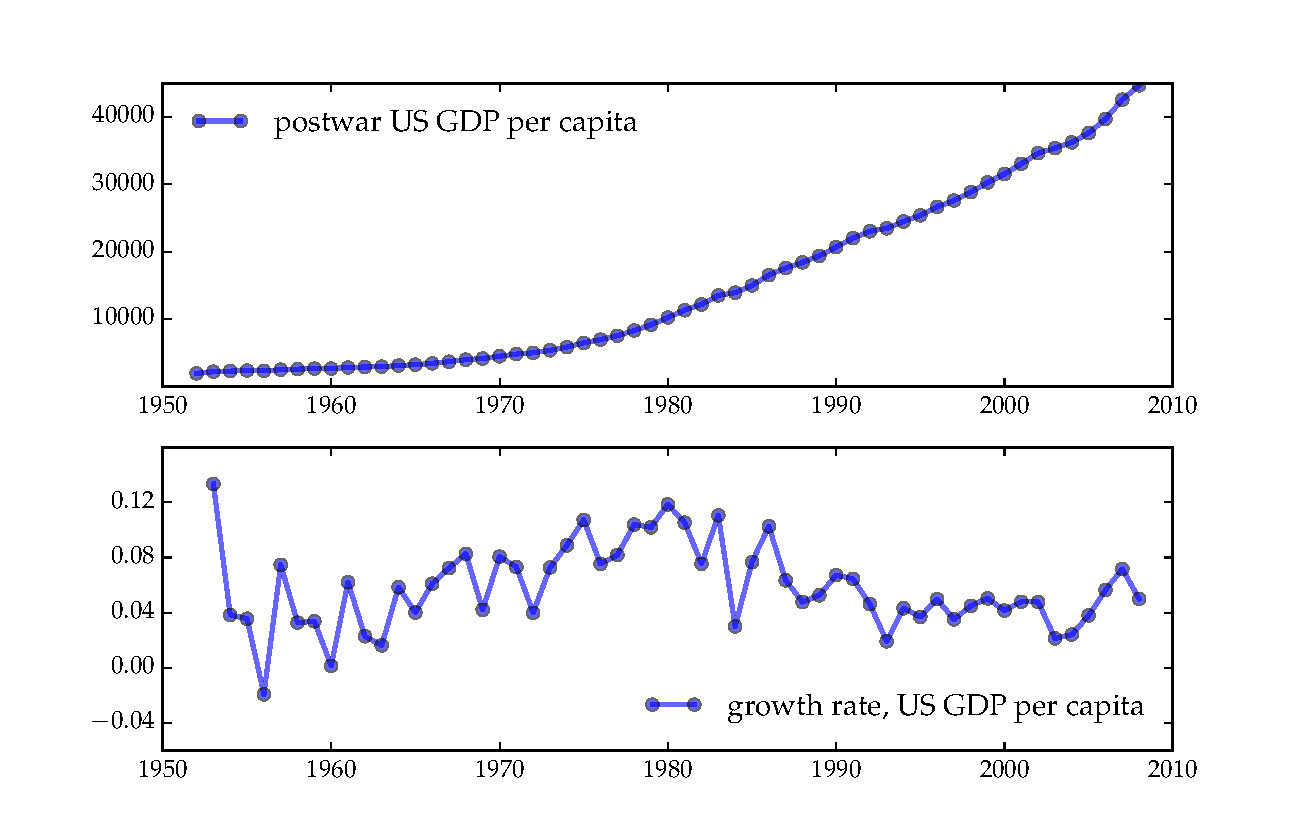
\includegraphics[trim={0 0.5em 0 1em}, clip]{gdp.pdf}}
        \caption{\label{f:gdp} Postwar US GDP per capita. Source: Penn World Tables}
        
    \end{figure}

\end{frame}

\begin{frame}

    \vspace{2em}
    The scalar Gaussian AR(1)  model can come close to the time-series of US GDP growth rates 
    %
    \begin{equation}
    \label{eq:sgar1}
    x_{t+1} = b + a x_t + c w_{t+1}
    \end{equation}
    %
    $\text{with } \{ w_t \} \iidsim \nN(0,1)
    \text{ and } x_0 \text{ given}$
    
    \vspace{1em}
    Here $a, b$, and $c$ are parameters, while $x_t$
    is called the \navy{state variable}

\end{frame}

\begin{frame}

    \vspace{2em}
    Equation for Gaussian AR(1) process an example of  \navy{stochastic difference equation}  
    
    \vspace{1em}
    The process $\{x_t\}$ it defines
    is called a stochastic process or \navy{stochastic recursive sequence} 
    
    \vspace{2em}
    A realization of the process is called a \navy{time series}
    
\end{frame}

\begin{frame}
    
    \vspace{2em}
    The dynamics of $\{x_t\}$ depends on the parameters:
    \begin{itemize}
     \item If $a$ is outside the interval
    $(-1,1)$, the series tend to diverge 
    
    \item  If $|a| < 1$, then
    the opposite is true
    
    \end{itemize}
    
    \vspace{1em}
    For example, for
    $a = 0.9$, after an initial
    burn in period where the series is affected by the initial condition $x_0$,
    the process settles down to random motion within a band (between about 5 and
    15 in this case)
        
\end{frame}

\begin{frame}

    \vspace{2em}
    \begin{figure}
       \begin{center}
        \scalebox{.60}{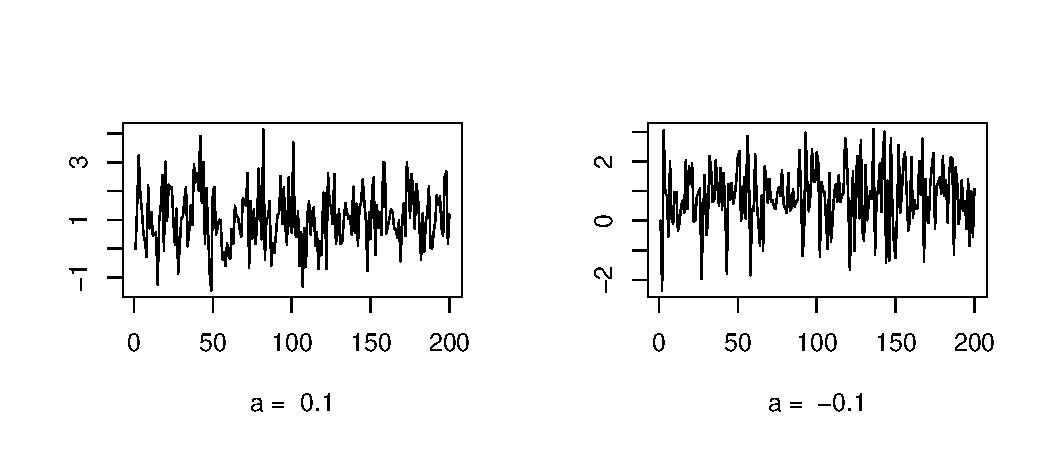
\includegraphics[trim=20 0 0 0, clip]{ar1_dynam_lec1.pdf}}
        \caption{Dynamics of the linear AR(1) model}
       \end{center}
    \end{figure}

\end{frame}

\begin{frame}

    \vspace{2em}
    \begin{figure}
       \begin{center}
        \scalebox{.60}{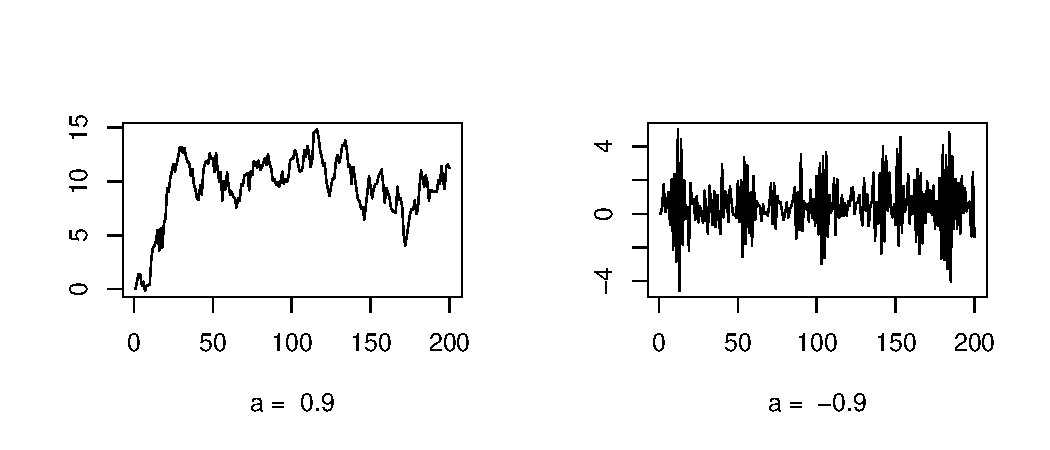
\includegraphics[trim=20 0 0 0, clip]{ar1_dynam_lec2.pdf}}
        \caption{\label{f:ar1_dynam} Dynamics of the linear AR(1) model}
       \end{center}
    \end{figure}

\end{frame}

\begin{frame}

    \vspace{2em}
    \begin{figure}
       \begin{center}
        \scalebox{.60}{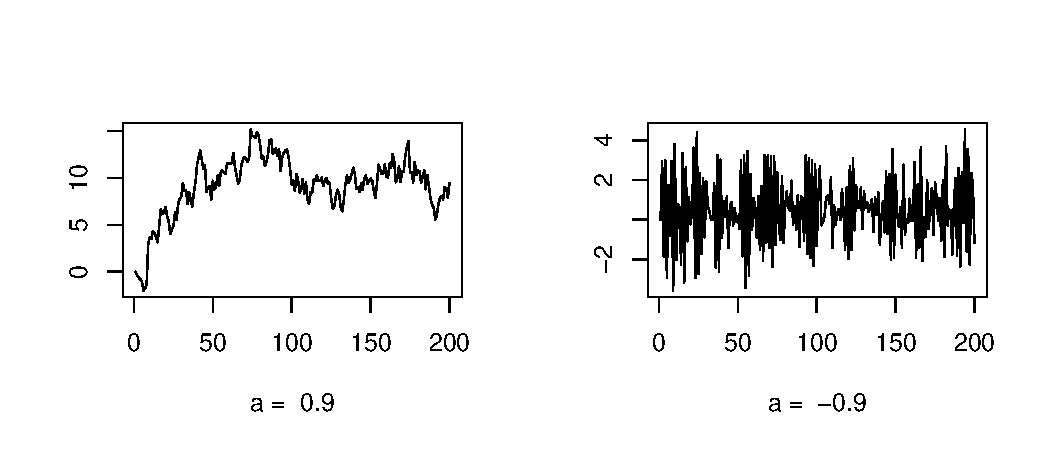
\includegraphics[trim=20 0 0 0, clip]{ar1_dynam_lec3.pdf}}
        \caption{Dynamics of the linear AR(1) model}
       \end{center}
    \end{figure}

\end{frame}



\begin{frame}

    \vspace{2em}
    Generalise the Gaussian AR(1) model by removing assumption that shocks are normal
    -- simply called AR(1) process

\end{frame}

\begin{frame}
    
    \vspace{2em}
    Generalize the scalar AR(1) model to $\RR^K$, yielding the vector
    AR(1) model, or VAR(1) model
    %
    \begin{equation}
    \label{eq:var1}
        \boldx_{t+1} = \boldb + \boldA \boldx_t + \boldC \boldw_{t+1}
    \end{equation}
    
    \vspace{1em}
    The sequence $\{ \boldw_t \}$ is {\sc iid} and satisfies
    $\EE \boldw_t = \boldzero$ and $\EE[\boldw_t\boldw_t'] = \boldI$
    
    If $\boldw_t$ is multivariate normal, then
    (\ref{eq:var1}) is called the Gaussian VAR(1). 
    
    The vector
    $\boldx_t$ is called the \navy{state vector} 
    
\end{frame}

\begin{frame}

    \vspace{2em}
    AR(p) model where $x_{t+1}$ is a linear function of previous p states
    
    \vspace{1em}
    AR(2) process has dynamics
%
    \begin{equation*}
        x_{t+1} = b + a x_t + \gamma x_{t-1} + w_{t+1}
    \end{equation*}

\end{frame}

%

\begin{frame}

    \vspace{2em}
    We can reformulate AR(2) as a first-order model 
    
    \vspace{1em}
    Define $y_t$ via $y_t = x_{t-1}$; the process can
    be expressed as
    %
    \begin{align*}
        x_{t+1}  &= b + a x_t + \gamma y_t + w_{t+1}  \\
        y_{t+1}  &= x_t
    \end{align*}
    
    and in matrix form as
    %
    \begin{equation*}
        \left( 
        \begin{array}{c}
            x_{t+1} \\
            y_{t+1} 
        \end{array}
        \right)
        = 
        b
        \left( 
        \begin{array}{c}
            1 \\
            0
        \end{array}
        \right)
        +
        \left( 
        \begin{array}{cc}
            a & \gamma \\
            1    & 0
        \end{array}
        \right)
        \left( 
        \begin{array}{c}
            x_t \\
            y_t 
        \end{array}
        \right)
        +
        \left( 
        \begin{array}{c}
            1 \\
            0
        \end{array}
        \right)
        w_{t+1}
    \end{equation*}
    
    This is a special case of the VAR(1) model in (\ref{eq:var1})
    
\end{frame}



\begin{frame}

    \vspace{2em}
    \vspace{10 mm}
    \begin{figure}
    \centering
    \scalebox{.4}{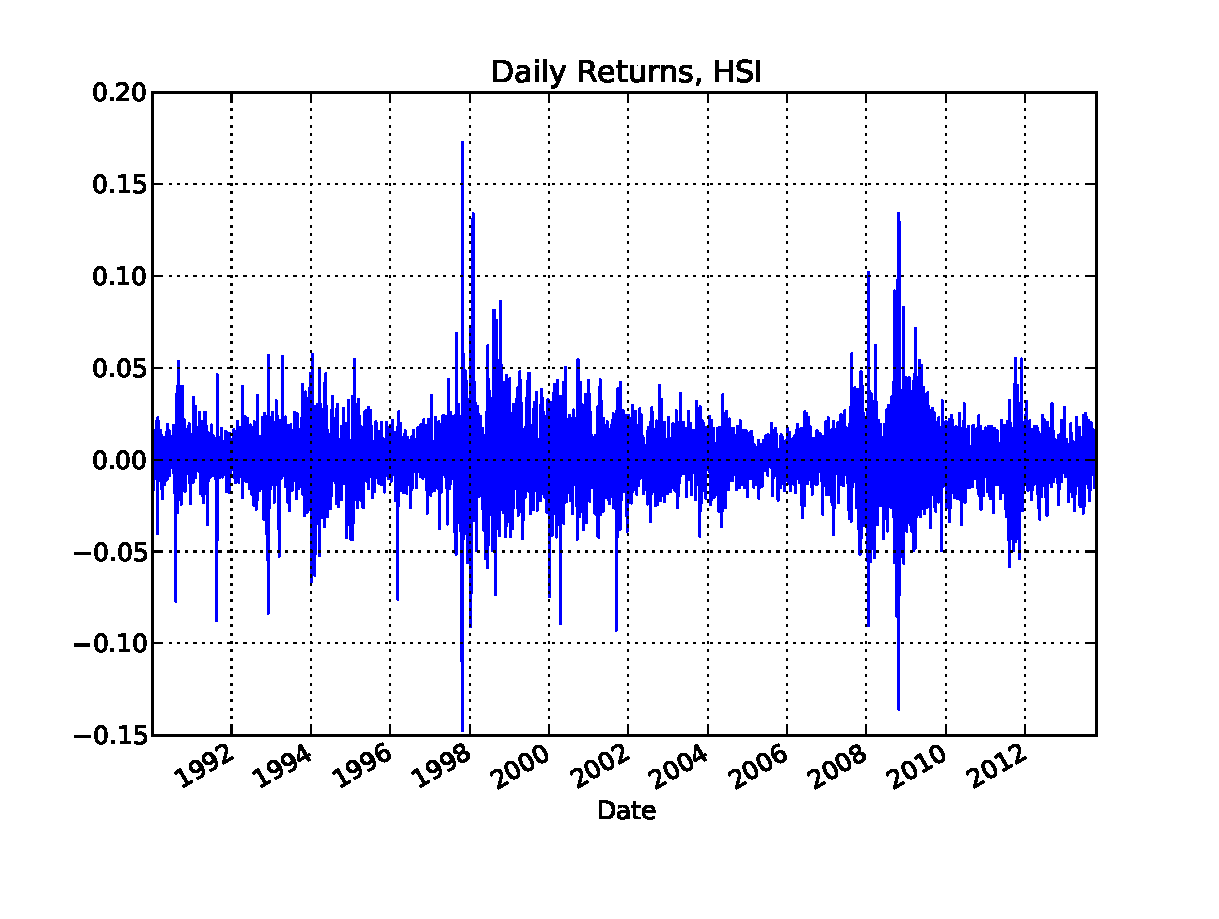
\includegraphics[trim={2em 2em 2em 2em}, clip]{hsi.pdf}}
    \caption{\label{f:hsi} Daily returns on the Hang Seng Index.  Source: Yahoo! Finance}
    
\end{figure}


\end{frame}

\begin{frame}

    \vspace{2em}
    Bursts of volatility in the Hang-Seng Index difficult to replicate
    without \emph{non-linearities}
    
    Need to model time-varying volatility in asset returns: consider $p$th
    order \navy{autoregressive conditional
    heteroskedasticity model} (ARCH($p$) model)
    %   
    \begin{equation}
        \label{eq:arch}
        x_{t+1} = (\alpha_0 + \alpha_1 x_t^2)^{1/2} w_{t+1}
        \quad \text{with} \quad \{ w_t \} \iidsim \nN(0,1)
    \end{equation}
    %
    and $\alpha_0 > 0$, $\alpha_1 \geq 0$
    
    \vspace{1em}
    Model contains time varying volatility $\sigma_{t+1}^2 =
    \alpha_0 + \alpha_1 x_t^2$
    
\end{frame}

\begin{frame}

    \vspace{2em}
    Still better fits to asset returns data can be obtained via \navy{Generalized ARCH models}
    
    \vspace{2em}
    The GARCH(1,1) process
    %
    \begin{align*}
        x_t &= \sigma_t w_t \\
        \sigma_{t+1}^2 &= \alpha_0 + \alpha_1 x_t^2 + \alpha_2 \sigma_t^2
    \end{align*}
    %
    Next period volatility depends on its own lagged state as well as $x_t$
    
\end{frame}

\section{Markov Processes}

\begin{frame}\frametitle{Markov Processes}
    
    \vspace{2em}
    Processes we have studied so far in this lecture are Markov processes 

    \vspace{.7em}
    Let $S\subset\RR^K$ and let
    $\bB(S)$ be the Borel subsets of $S$  
    
    The primitive of a discrete
    time Markov process on $S$ is a \navy{stochastic kernel} or \navy{transition
    probability function} $Q \colon S \times \bB(S) \to [0,1]$ such that
    %
    \begin{enumerate}
    \item $Q(\bolds, \cdot)$ is a probability measure over $\bB(S)$ for all
        $\bolds \in S$ and
    \item $g(\bolds) := Q(\bolds, B)$ is $\bB$-measurable for each $B \in \bB(S)$
    \end{enumerate}
    %
    $S$ is called the \navy{state space} of the model 
    
\end{frame}

\begin{frame}

    \vspace{2em}
    $Q$ and some initial
    distribution $P_0$ generate a Markov process $\{\boldx_t\}$ via
    
    \vspace{0.6em}
    \begin{algorithmic}[1]
        \State draw $\boldx_0$ from $P_0$
        \For{$t$ in $0, 1, 2, \ldots$}
            \State draw $\boldx_{t+1}$ from the distribution $Q(\boldx_t, \cdot)$
        \EndFor
    \end{algorithmic}

    The generated sequence $\{\boldx_t\}$ also called a \navy{sample path} for $Q$
    
\end{frame}

\begin{frame} 

    \vspace{2em}
    The canonical stochastic difference
    equation for a \navy{first-order Markov process} takes the form 
    %
    \begin{equation}
        \label{eq:amp}
        \boldx_{t+1} = G(\boldx_t, \boldw_{t+1})
        \quad \text{with} \quad
        \lL(\boldx_0) = P_0
    \end{equation}
    
    \vspace{1em}
    The sequence of $\RR^M$-valued shocks $\{\boldw_t\}_{t \geq 1}$ is {\sc iid} 
    has common distribution $\Psi$
    
    $G$ is a given $\bB$-measurable function 
    
    Initial condition $\boldx_0$ and the shocks $\{\boldw_t\}_{t \geq 1}$ also independent
    
\end{frame}

\begin{frame}

    \vspace{1em}
    Stochastic difference equation specifies the process $\{x_{t}\}$ and stochastic kernel 
    %
    \begin{equation*}
        Q(\bolds, B) = \PP\{G(\bolds, \boldw_{t+1}) \in B\}
        \qquad (\bolds \in S, \; B \in \bB(S))
    \end{equation*}
    
    \vspace{2em}
    Recalling that $\Psi$ is the distribution of $\boldw_{t+1}$,
    the stochastic kernel can also be written as 
    %
    \begin{equation*}
        Q(\bolds, B) 
        = \Psi \left\{\boldw \in \RR^M \; : \; G(\bolds, \boldw) \in B \right\}
    \end{equation*}
    
\end{frame}

\begin{frame}

    \vspace{2em}
    \Eg
    For the ARCH(1) model of \eqref{eq:arch}, the stochastic kernel is
    %
    \begin{equation*}
        Q(s, B) = \PP\{ (\alpha_0 + \alpha_1 s^2)^{1/2} w_{t+1} \in B \}
    \end{equation*}
    %
    when $w_{t+1}$ is standard normal

\end{frame}

\begin{frame}

    \vspace{2em}
    Repeated substitution gives
    %
    \begin{align*}
        \boldx_1 & = G(\boldx_0, \boldw_1) \\
        \boldx_2 & = G(G(\boldx_0, \boldw_1), \boldw_2) \\
        \boldx_3 & = G(G(G(\boldx_0, \boldw_1), \boldw_2),\boldw_3)
    \end{align*}
    %
    and so on...
    
    \vspace{1em}
    The state vector $\boldx_t$ can be written as a function of $\boldx_0$ and the shocks
    $\boldw_1,\ldots,\boldw_t$ for any $t$; there
    exists a function $H_t$ such that 
    %
    \begin{equation}
        \label{eq:xaft}
        \boldx_t = H_t(\boldx_0, \boldw_1, \boldw_2,\ldots, \boldw_t)
    \end{equation}
    %

\end{frame}

\begin{frame}

    \vspace{2em}
    \Eg
    \label{eg:sar1}
    For the scalar linear AR(1) process \eqref{eq:sgar1}
    we can write the right-hand side of (\ref{eq:xaft}) explicitly as 
    %
    \begin{equation}
        \label{eq:ar1ft}
        x_t = b \sum_{k=0}^{t-1} a^k 
            + \sum_{k=0}^{t-1} a^k c w_{t-k} + a^t x_0
    \end{equation}
    %
    This is called the \navy{moving average representation} of $x_t$
    
\end{frame}

\begin{frame}

    \Fact\textcolor{Brown}{\eqref{ET-fa:aamp}}
    For the process \eqref{eq:amp}, the pair $\boldx_t$ and 
    $\boldw_{t+k}$ are independent for all $k \geq 1$ 
    
\end{frame}


\begin{frame}

    \vspace{2em}
    If $Q(\bolds, \cdot)$ is absolutely continuous for all $\bolds$, 
    then define the corresponding \navy{stochastic density kernel} or the \navy{transition
    density} 
    %
    \begin{equation*}
        \label{eq:td}
        q(\bolds, \cdot) := \text{ the density of } Q(\bolds, \cdot)
        \text{ for all } \bolds \in S
    \end{equation*}
    
    \vspace{1em}
    The function $q(\bolds, \cdot)$ is the conditional density of
    $\boldx_{t+1}$ given $\boldx_t = \bolds$
    
    Heuristically, $q(\bolds, \bolds') \diff \bolds'$ is the
    probability of transitioning from $\bolds$ to $\bolds'$ in one step
    
\end{frame}


\begin{frame}

    \vspace{2em}
    \Eg
        Recall the ARCH(1) process, with stochastic kernel 
         \begin{equation*}
            Q(s, B) = \PP\{ (\alpha_0 + \alpha_1 s^2)^{1/2} w_{t+1} \in B \}
        \end{equation*}
        
        The transition density $q(s, \cdot)$ is the density
        of $y = (\alpha_0 + \alpha_1 s^2)^{1/2} w_{t+1}$ when
        $\lL(w_{t+1}) = \nN(0, 1)$.  Hence
        %
        \begin{equation*}
            \label{eq:arch_td}
            q(s, s') 
            = 
            \frac{1}{\sqrt{2 \pi \sigma_s^2}}
               \exp \left\{ - 
               \frac{(s')^2}{2\sigma^2_s} \right\} 
            \quad \text{where} \quad
            \sigma^2_s := \alpha_0 + \alpha_1 s^2
        \end{equation*}
    %
\end{frame}

\begin{frame}

    \vspace{2em}
    Consider the generic process 
    $\boldx_{t+1} = G(\boldx_t, \boldw_{t+1})$, where 
    $\lL(\boldx_0) = P_0$ and $\{\boldw_t\}$ is {\sc iid} on $\RR^M$ with common
    distribution $\Psi$
    
    The \navy{marginal distribution of the state vector} is
    $\lL(\boldx_t)$ 
    
    \vspace{1em}
    Since $\boldx_t$ is a well-defined random vector, $\lL(\boldx_t)$ is also well-defined, and we denote it by
    %
    \begin{equation*}
        P_t(B) = \PP\{\boldx_t \in B\}
        \qquad (B \in \bB(S))
    \end{equation*}
    %
    \end{frame}

\begin{frame}

    \vspace{2em}
    \Eg Consider the Gaussian AR(1) process
        
        Suppose $\lL(x_0)= \nN(\mu_0,
        \sigma_0^2)$, where $\mu_0$ and $\sigma_0$ are given constants and $x_0$
        is independent of the shock process $\{w_t\}$
    
        Combining the moving average representation of $x_t$ we have $P_t = \nN \left(
                    \mu_t, \, \sigma_t^2
                \right)$ 
        %
        \begin{equation*}
            \text{where} \quad
            \mu_t := b \sum_{k=0}^{t-1} a^k + a^t \mu_0
            \; \text{ and } \;
            \sigma^2_t := \sum_{k=0}^{t-1} a^{2k} c^2  + a^{2t} \sigma_0^2
        \end{equation*}
        %
\end{frame}

\begin{frame}

    \begin{figure}
        \centering
        \scalebox{.42}{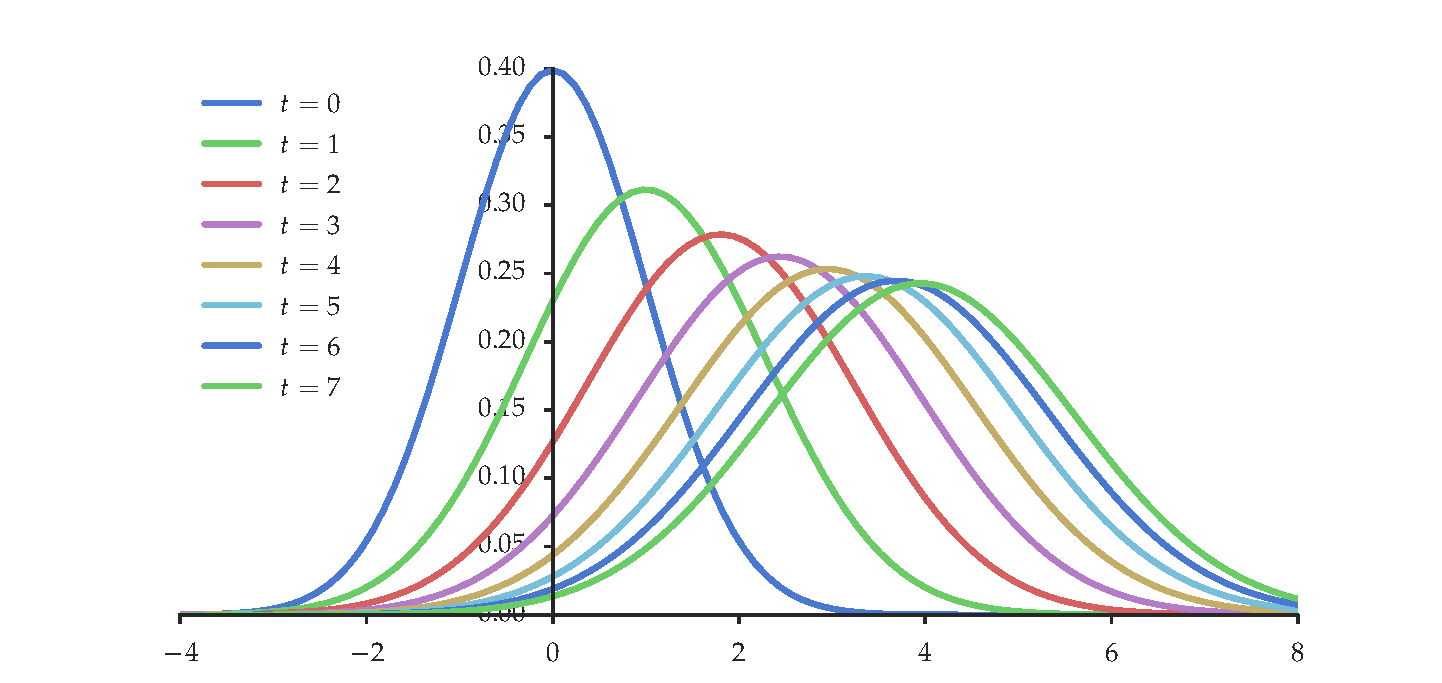
\includegraphics[trim={0 0em 0 2em}, clip]{norm_den_seq.pdf}}
        \caption{\label{f:norm_den_seq} Sequence of marginal densities for the Gaussian AR(1)
        process when $\mu_0=0$, $\sigma_0 = b = c =1$ and $a = 0.8$}
    \end{figure}
    \end{frame}

\begin{frame}

    \vspace{2em}
    For general Markov processes, tracking evolution of first two moments is more complicated
    
    \vspace{1em}
    \Fact\textcolor{Brown}{\eqref{ET-fa:rdli}}
        The marginal distributions of a Markov process with stochastic kernel $Q$
        obey the recursion
        %
        \begin{equation}
            \label{eq:rdli}
            P_{t+1}(B) = \int Q(\bolds, B) P_t(\diff  \bolds)
            \qquad (B \in \bB(S),\; t \geq 0)
        \end{equation}
    
\end{frame}

\begin{frame}

    \vspace{2em}
    \Fact\eqref{ET-fa:detsmp}
        If $Q(\bolds, \cdot)$ is absolutely continuous for all $\bolds \in S$,
        then $P_t$ is absolutely continuous for all $t \geq 1$.  Letting $p_t$
        be the corresponding density, the sequence $\{p_t\}$ satisfies 
        %
        \begin{equation}
            \label{eq:rdli2}
            p_{t+1}(\bolds') = \int q( \bolds, \bolds') p_t(\bolds) \diff \bolds
            \qquad (B \in \bB(S),\; t \geq 1)
        \end{equation}
        %
        where $q$ is the transition density corresponding to $Q$

\end{frame}

\begin{frame}

    \vspace{2em}
    \Fact (7.2.4) Let $\{\boldx_t\}$ be a Markov process with transition density $q$ and
    initial density $p_0$.
    Under the conditions of fact~\ref{ET-fa:detsmp} in ET, the joint density $p_T$ of
    $\boldx_0, \ldots, \boldx_T$ is
    %
    \begin{equation}
        \label{eq:jftd}
        p_T(\bolds_0, \ldots, \bolds_T) 
        = p_0(\bolds_0) \prod_{t=0}^{T-1} q(\bolds_t, \bolds_{t+1} ) 
    \end{equation}
    %
   \Prf First, factor the joint density into 
    %
    \begin{equation*}
        p_T(\bolds_0, \ldots, \bolds_T) 
        = p_0(\bolds_0) \prod_{t=0}^{T-1} p(\bolds_{t+1} \given \bolds_t, \ldots, \bolds_0) 
    \end{equation*}
    %
    This is the expression for the joint density of a general stochastic process.  With first order Markov property, 
    $p(\bolds_{t+1} \given \bolds_t, \ldots, \bolds_0)$ reduces to $p(\bolds_{t+1}
    \given \bolds_t)=q(\bolds_t, \bolds_{t+1})$
    
\end{frame}

\begin{frame}\frametitle{Stationarity of Markov Processes}

    \vspace{2em}
    Marginals $\{P_{t}\}$ of Gaussian AR(1) process can change over time, but difference
    between successive distributions diminishing over time
     
    \vspace{1em}
    Recall $P_t = \nN(\mu_t,
    \sigma^2_t)$, where $\mu_t$ and $\sigma^2_t$. Provided  $|a| < 1$, sequences converge
    %
    \begin{equation*}
        \mu_t \to \mu_{\infty} := \frac{b}{1 - a}
        \quad \text{and} \quad
        \sigma^2_t \to \sigma^2_{\infty} := \frac{c^2}{1 - a^2}
    \end{equation*}
    %
    Let $P_\infty$ denote the limiting distribution
    %
    \begin{equation}
        \label{eq:sdsg}
        P_\infty 
        = \nN(\mu_\infty, \sigma_\infty^2)
        = \nN \left[ \frac{b}{1 - a}, \frac{c^2}{1 - a^2} \right]
    \end{equation}
    
\end{frame}

\begin{frame}
 
    \begin{figure}
        \centering
        \scalebox{.40}{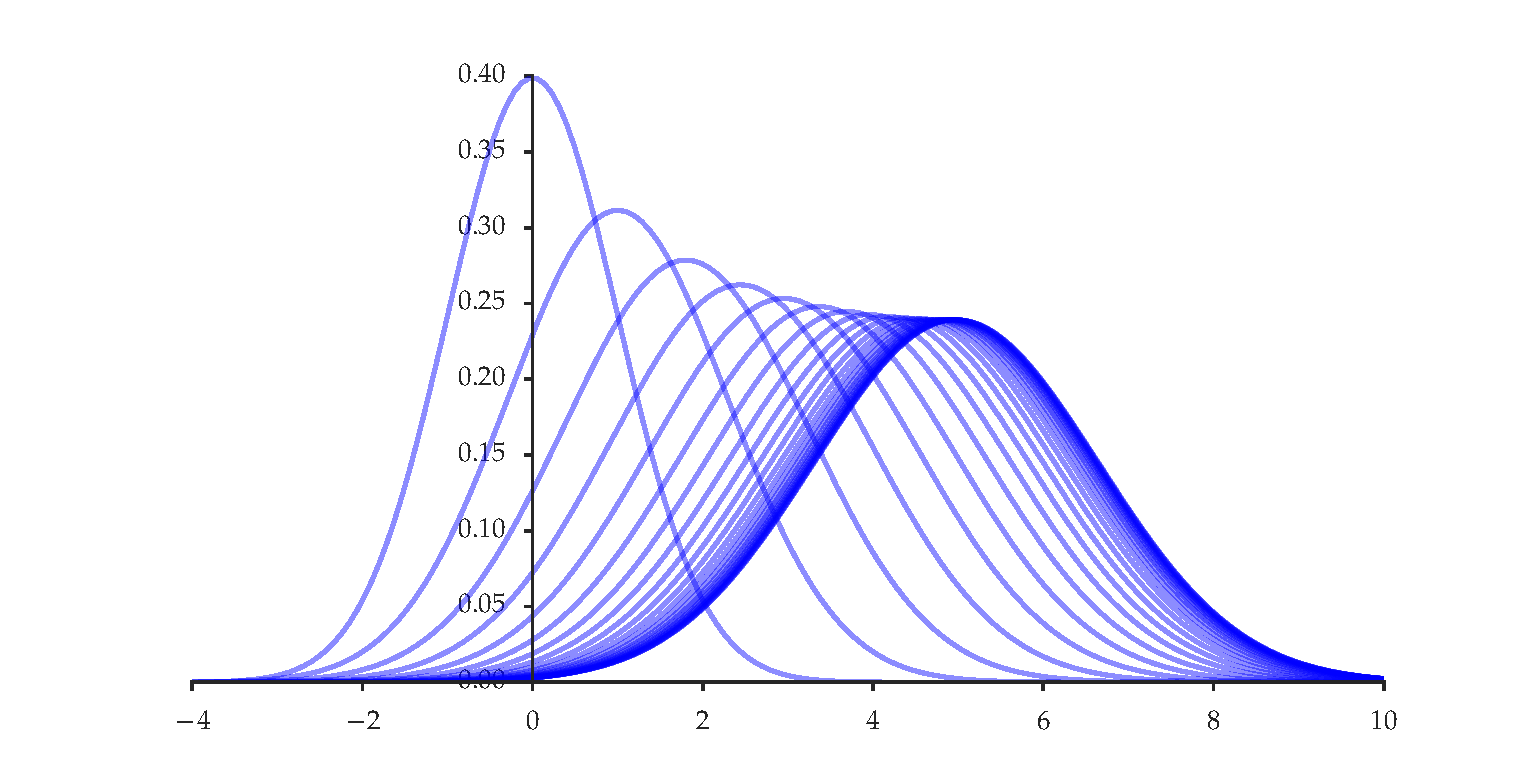
\includegraphics[trim={0 0em 0 2em}, clip]{long_norm_den_seq.pdf}}
        \caption{\label{f:long_norm_den_seq} Convergence of marginal densities, Gaussian AR(1) case}
    \end{figure}
 
\end{frame}

\begin{frame}

    \vspace{2em}
    Limiting distribution is an example of a stationary distribution 
    
    \vspace{1em}
    A \navy{stationary distribution} for a Markov process on $S$ with stochastic kernel
    $Q$ is any distribution $P_\infty$ on $S$ satisfying
    %
    \begin{equation*}
        P_\infty(B) = \int Q(\bolds, B) P_\infty(\diff \bolds)   
        \qquad \text{for all } B \in \bB(S)
    \end{equation*}
    %
    Comparing with the recursion $P_{t+1}(B) = \int Q(\bolds, B) P_t(\diff \bolds)$,
    the definition of stationarity of $P_\infty$ means precisely 
    %
    \begin{equation*}
    \lL(\boldx_t) = P_\infty
    \; \implies \; 
    \lL(\boldx_{t+1}) = P_\infty
    \end{equation*}
    %
    Any process starting at $P_\infty$ will be {\sc iid}
    
\end{frame}

\begin{frame}

    \vspace{2em}
        \Fact\eqref{ET-fa:idmp} 
        Let $\{\boldx_t\}$ be a Markov process with stationary distribution
        $P_{\infty}$. If $\lL(\boldx_0) =  P_{\infty}$, then $\{\boldx_t\}$ is
        a stationary stochastic process, with $\lL(\boldx_t) = P_{\infty}$ for all $t$
    
    \vspace{1em}
    \Eg
        Consider the scalar Gaussian linear AR(1) process from \eqref{eq:sgar1}.
        If $|a| < 1$ and $\lL(x_0) = P_\infty$, where $P_\infty$ is as in
        \eqref{eq:sdsg}, then $\{x_t\}$ is stationary
        
\end{frame}

\begin{frame}

    \vspace{2em}
    \Fact (7.2.6)
    If $Q(\bolds, \cdot)$ is absolutely continuous for all $\bolds \in S$
    with transition density $q(\bolds, \cdot)$, then every stationary
    distribution $P_\infty$ is absolutely continuous, and its density
    $p_\infty$ satisfies
    %
    \begin{equation}
        \label{eq:dsdist}
        p_{\infty}(\bolds') 
        = \int q(\bolds, \bolds' ) p_{\infty}(\bolds) \, \diff \bolds
        \quad \text{for all } \bolds' \in S
    \end{equation}
    %
\end{frame}

\begin{frame}
    
    \vspace{2em}
    Not every Markov process has a stationary distribution
    
    \vspace{1em}
    Recall linear scalar AR(1) model $x_{t+1} = b + a x_t + c w_{t+1}$
    \begin{itemize}
    \item the
    marginal variance evolves according to $\sigma^2_{t+1} = a^2 \sigma_t^2 +
    c^2$
    \end{itemize}
    
    \vspace{1em}
    If $|a| \geq 1$, then this sequence diverges since the variance is
    not constant
    
\end{frame}

\begin{frame}

    \vspace{2em}
    A sufficient condition for existence  
    
    The condition we give slightly specializes the famous Krylov--Bogolyubov theorem
    
    \vspace{1em}
    It uses the notion of a \navy{coercive} function, which is any nonnegative
    function $V$ on the state space $S$ such that 
    %
    \begin{equation*}
        C_\gamma := \setntn{\bolds \in S}{V(\bolds) \leq \gamma}
    \end{equation*}
    
    is a compact subset of $S$ for all $\gamma \in \RR$
    
\end{frame}

\begin{frame}

    \vspace{2em}
    \Eg
    If $S = \RR^K$ and $V(\bolds) = \| \bolds \|$, then $V$ is coercive on
    $S$.  Indeed, for this function, each $C_\gamma$ is a closed sphere
    centered on the origin.  Closed and bounded subsets of $\RR^K$ are compact. 

    \vspace{1em}
    \Eg
    If $S = \RR$ and $V(s) = s^2$, then $V$ is coercive on
    $S$.  To see this, just observe that $C_\gamma = [-\sqrt{\gamma}, \sqrt{\gamma}]$.
    This is a closed, bounded subset of $S$.
  

\end{frame}
 
\begin{frame}

    \vspace{2em}
    \Thm{\textcolor{Brown}{\bf\eqref{ET-t:esd}}}
    Let $\boldx_{t+1} = G(\boldx_t, \boldw_{t+1})$ be the process on $S$
    defined in \eqref{eq:amp}.   If
    %
        \begin{enumerate}
            \item $\bolds \mapsto G(\bolds, \boldw)$ is continuous for each fixed
                $\boldw \in \RR^M$, and
            \item there exists a coercive function $V$ on $S$ and 
                constants $\lambda$ and $L$ such that $0 \leq \lambda < 1$ and
                %
                \begin{equation}
                    \label{eq:cwrtc}
                    \EE  V[ G(\bolds, \boldw_{t+1} ) ] 
                    \leq \lambda V(\bolds) + L
                    \qquad (\bolds \in S)
                \end{equation}
                %
        \end{enumerate}
    %
    then the Markov process has at least one stationary distribution.
    
\end{frame}

\begin{frame}

    \vspace{2em}
    Condition \eqref{eq:cwrtc} is an example of a \navy{drift condition}. 
    One way to understand it is to write it as 
    %
    \begin{equation*}
        \frac{\EE  V[ G(\bolds, \boldw_{t+1} )  ] }{V(\bolds)}
            \leq \lambda + \frac{L}{V(\bolds) }
    \end{equation*}
    %
    As we move ``away from the center" of the state space, $V(\bolds)$ becomes
    large, and the term on the right is eventually $< 1$
    
    \vspace{2em}
    Looking at the left hand side, the value attached to the state by $V$ is expected
    to decrease, suggesting movement away from the ``edges" of the state space 
    and back towards the center
    
\end{frame}

\begin{frame}

    \vspace{2em}
    \Eg Consider again the ARCH(1) process $x_{t+1} = (\alpha_0 + \alpha_1
        x_t^2)^{1/2} w_{t+1}$ from \eqref{eq:arch}, where, as usual $\alpha_0 > 0$
        and $\alpha_1 \geq 0$.  Let $S = \RR$.  If $\alpha_1 < 1$, then
        this process has a stationary distribution on $S$.  To see this, observe
        that
        %
        \begin{equation*}
            G(s, w) = (\alpha_0 + \alpha_1 s^2)^{1/2} w
            \qquad (s, w \in \RR)
        \end{equation*}
        %
        is continuous in $s$ for each fixed $w$.  Moreover, we showed $V(s) = s^2$ is
        coercive on $S$, and 
        %
        \begin{equation}
            \label{eq:archas}
            \EE G(s, w_{t+1})^2  
            = (\alpha_0 + \alpha_1 s^2) \EE w_{t+1}^2
            = \alpha_0 + \alpha_1 s^2
        \end{equation}
        %
        Hence \eqref{eq:cwrtc} holds with equality when $V(s) :=s^2$, $\lambda :=\alpha_1$ and
        $L := \alpha_0$

\end{frame}

\begin{frame}
    
    \vspace{2em}
    \Thm\eqref{ET-t:umspt} 
    \label{t:umspt}
    Let $\{\boldx_t\}$ be a Markov process on $S$ with stochastic kernel $Q$.
    Suppose $Q(\bolds, \cdot)$ is absolutely continuous for all $\bolds
    \in S$ and let $q(\bolds, \cdot )$ be the corresponding transition
    density.  If
    %
    \begin{enumerate}
        \item[(a)] $q$ is strictly positive and continuous on $S \times S$, and
        \item[(b)] there exists a coercive function $V$ on $S$ and 
            constants $\lambda$ and $L$ such that $0 \leq \lambda < 1$ and
            %
            \begin{equation*}
                \int V(\bolds') q(\bolds, \bolds' ) \diff  \bolds'
                \leq \lambda V(\bolds) + L
                \qquad (\bolds \in S)
            \end{equation*}
            %
    \end{enumerate}
    %
    then the following statements are true (continued on the next slide)
    
\end{frame}

\begin{frame}

    \vspace{2em}
    \Thm\eqref{ET-t:umspt}(cont.) 
    %
    \begin{enumerate}
        \item $Q$ has a unique stationary distribution $P_\infty$ with
            density $p_\infty$.
        \item $P_t \tow P_\infty$ as $t \to \infty$ for all initial $P_0$.
        \item  If $h \colon S \to \RR$ is $\bB$-measurable 
            and $\int |h(\bolds)| p_{\infty}(\bolds)\diff \bolds < \infty$,
            then
            %
            \begin{equation}
                \label{eq:mllnr}
                \frac{1}{T} \sum_{t=1}^T h(\boldx_t) 
                \toprob 
                \int h(\bolds) p_{\infty}(\bolds) \diff \bolds
                \quad \text{as} \quad
                T \to \infty
            \end{equation}
            %
        \item If, in addition, $h^2 \leq V$, then there exists a 
            $\sigma^2_h \geq 0$ such that 
            %
            \begin{equation}
                \label{eq:mkclt}
                \sqrt{T}
                \left\{
                    \frac{1}{T} \sum_{t=1}^T h(\boldx_t) -
                    \int h(\bolds) p_{\infty}(\bolds) \diff \bolds
                \right\}
                \tod \nN(0, \sigma^2_h)
                \quad 
            \end{equation}
            $\quad \text{as}\quad 
                T \to \infty$
            %
    \end{enumerate}
    %
\end{frame}



\begin{frame}

    \vspace{2em}
    \Fact\eqref{ET-fa:gsmp}
        \label{fa:gsmp}
        Let $\boldx_{t+1} = g(\boldx_t) + \boldw_{t+1}$ be the additive shock
        process on $\RR^K$ from \eqref{ET-eq:ampadd}.  If $\EE \|\boldw_t\|$ is
        finite, $g$ is continuous, the density $\psi$ of $\boldw_t$ is continuous
        and positive everywhere on $\RR^K$, and there exist constants $\lambda$
        and $L$ such that $0 \leq \lambda < 1$ and
        %
        \begin{equation}
            \label{eq:drift}
            \| g(\bolds) \| \leq \lambda \| \bolds \| + L
            \quad \text{ for all } \bolds \in \RR^K
        \end{equation}
        %
        then the conditions of theorem~\ref{ET-t:umspt} are satisfied.  
    
\end{frame}

\begin{frame}
    
    \vspace{2em}
    \Prf  Recall the transition density
    satisfies $q(\bolds, \bolds' ) = \psi(\bolds' - g(\bolds))$ 
    
    Since
    $\psi$ is assumed continuous and positive on $\RR^K$, condition (a) in
    theorem~\ref{ET-t:umspt} is satisfied
    
    Condition (b) is also satisfied because,
    taking $\lambda$ and $L$ as in \eqref{eq:drift}
    %
    \begin{multline*}
        \int \|\bolds'\| q(\bolds, \bolds' ) \diff  \bolds'
        \\ = \EE \|g(\bolds) + \boldw_{t+1} \| 
        \leq \lambda \| \bolds \| + L + \int \|\boldw\| \psi(\boldw) \diff \boldw
    \end{multline*}
\end{frame}

\begin{frame}

    \vspace{2em}
    \Eg Gaussian VAR(1)
    %
    \begin{equation}
        \label{eq:var12}
        \boldx_{t+1} = \boldb + \boldA \boldx_t + \boldC \boldw_{t+1}
    \end{equation}
    %
    In this case, $g(\bolds) = \bolda + \boldA \bolds$, and
    %
    \begin{equation*}
        \|g(\bolds)\| 
        = \| \boldb + \boldA \bolds\|
        \leq \| \boldb \|  + \| \boldA \bolds\|
        \leq \| \boldb \|  + \| \boldA \| \| \bolds\|
    \end{equation*}
    
    \vspace{.7em}
    Thus, we can apply fact~\ref{ET-fa:gsmp} to obtain asymptotic stability 
    and LLN and CLT results
    whenever the matrix norm of $\boldA$ satisfies $\|\boldA \| < 1$
    
\end{frame}

\begin{frame}

    \vspace{2em}
    We have a better result 
    
    \Fact (7.2.8)
    For the VAR process \eqref{eq:var12}, the conclusions of
    theorem~\ref{ET-t:umspt} hold with $V = \| \cdot \|$ whenever $\rho(\boldA) <
    1$
    
    
    Here $\rho(\boldA)$ is the spectral radius of $\boldA$.  
    
    Taking expectations across \eqref{eq:var12}, the mean
    $\boldmu_{\infty}$ must satisfy $\boldmu_{\infty} = \boldb + \boldA
    \boldmu_{\infty}$.  
    
    Apply the Neumann series lemma (page~\pageref{ET-t:nms} in ET)
    %
    \begin{equation*}
        \boldmu_\infty 
        = (\boldI - \boldA)^{-1} \boldb 
        = \sum_{i=0}^{\infty} \boldA^i  \boldb 
    \end{equation*}
    
\end{frame}
    
\begin{frame}[fragile]
        
    \vspace{2em}
    Let $\boldSigma_\infty$ be 
    the asymptotic variance (i.e., the variance--covariance matrix of the
    stationary distribution); $\boldSigma_\infty$ must satisfy
    %
    \begin{equation*}
        \boldSigma_\infty = \boldA \boldSigma_\infty \boldA^\T + \boldC \boldC^\T
    \end{equation*}
    %
    This is an example of a \navy{discrete time Lyapunov equation}

    Under the condition
    $\rho(\boldA) < 1$, we can be solve by iteration or by using existing
    numerical solvers
    
    \small \begin{juliacode}
using QuantEcon

A = [0.8 -0.2; 
    -0.1 0.7]
C = [0.5 0.4;
     0.4 0.6]

solve_discrete_lyapunov(A, C * C')
    \end{juliacode}

\end{frame}

\section{Martingales}

\begin{frame}\frametitle{Martingales}
    
    \vspace{2em}
    A stochastic process evolving over time such that best guess of 
    next value given current value is current value

    \vspace{1em}
    Let $\{\fF_t\}$ be a sequence of information sets

    The sequence $\{\fF_t\}$ is called a \navy{filtration} if $\fF_t \subset
    \fF_{t+1}$ for all $t$

    \vspace{1em}
    Intuition: reflects idea that more information is revealed over time
    
\end{frame}
    
\begin{frame}

    \vspace{2em}
    \Eg Let $\{\boldx_t\}$ be a sequence of random vectors, and let
        %
        \begin{equation*}
            \fF_0 := \emptyset, \; \;
            \fF_1 := \{\boldx_1\}, \; \;
            \fF_2 := \{\boldx_1, \boldx_2\}, \; \;
            \cdots
        \end{equation*}
    
    Then $\{\fF_t\}$ is a filtration called the filtration generated by $\{\textbf{x}_{t}\}$
    
\end{frame}



\begin{frame}

    \vspace{2em}
    Let 
    %
    \begin{itemize}
        \item $\{m_t\}$ be a sequence of RVs (scalar stochastic process)
        \item $\{\fF_t\}$ be a filtration
    \end{itemize}

    We say $\{m_t\}$ is \navy{adapted} to the filtration $\{\fF_t\}$ if
    $m_t$ is $\fF_t$-measurable for every $t$

    \vspace{1em}
    Intuition: If we know $\fF_t$ then we know $m_t$
    
\end{frame}

\begin{frame}

    \vspace{2em}
    \Eg If $\{\fF_t\}$ is the filtration defined by 
        %
        \begin{equation*}
            \fF_0 := \emptyset, \; \;
            \fF_1 := \{x_1\}, \; \;
            \fF_2 := \{x_1, x_2\}, \; \;
            \fF_3 := \{x_1, x_2, x_3\}, \;\;
            \cdots
        \end{equation*}
        %
        and $m_t := t^{-1} \sum_{j=1}^t x_j$, then $\{m_t\}$ is adapted to
        $\{\fF_t\}$
        
\end{frame}

\begin{frame}

    \vspace{2em}
    \Fact\textcolor{Brown}{\eqref{ET-fa:emfv}}
        If $\{m_t\}$ is adapted to filtration $\{\fF_t\}$, then $\EE[m_t \given \fF_{t+j}] =
        m_t$ for any $j \geq 0$
        
    \Prf
        We know
        \begin{itemize}
            \item $m_t$ is $\fF_t$-measurable
            \item If $j \geq 0$, then $\fF_t \subset \fF_{t+j}$
            \item If $\gG \subset \hH$, then $\gG$-measurable implies
                $\hH$-measurable
            \item If $y$ is $\hH$-measurable, then $\EE[y \given \hH] = y$
        \end{itemize}
        The result follows
        
\end{frame}


\begin{frame}
    
    \vspace{2em}
    Let $\{m_t\}$ be a sequence of random variables 
    %
    \begin{itemize}
        \item adapted to a filtration $\{\fF_t\}$
        \item having finite first moment
    \end{itemize}
    
    \vspace{1em}
    We say that $\{m_t\}$ is a \navy{martingale} with respect to $\{\fF_t\}$ if 
    %
    \begin{equation*}
        \EE [ m_{t+1} \given \fF_t] = m_t 
        \quad \text{for all} \quad t
    \end{equation*}
    %
    We can simplify the expression $\EE [ m_{t+1} \given \fF_t]$ to $\EE_{t}[x_{t+1}]$
    when the filtration is understood
    
\end{frame}


\begin{frame}

    \vspace{2em}
    \Eg Let $\{\eta_t\}$ be {\sc iid} with $\EE[\eta_1] = 0$ and define $m_t := \sum_{j=1}^t \eta_j$
    and let $\fF_t := \{\eta_1, \ldots, \eta_t\}$
    
    The sequence $\{m_t\}$ is a martingale with respect to $\{\fF_t\}$
    
    From the definitions, $\{m_t\}$ will be adapted to $\{\fF_t\}$. Moreover
    %
    \begin{equation*}
        \EE[ m_{t+1} \given \fF_t]  
         =  \EE[  m_t + \eta_{t+1} \given \fF_t] 
         =  m_t + \EE[ \eta_{t+1} \given \fF_t]
    \end{equation*}
    
\end{frame}


\begin{frame}
    
    \vspace{2em}
    \Eg Consider an Euler equation of the form
    %
    \begin{equation*}
        u'(c_t) = \EE_t \left[ \frac{1+r_{t+1}}{1+\rho} \cdot u'(c_{t+1}) \right]
    \end{equation*}
    
    \vspace{1em}
    Where $u$ is a utility function, $r_t =$ the interest rate and $\rho =$ a discount factor.
    $\EE_t[\cdot] = \EE[\cdot \given \fF_t]$, where $\fF_t =$ information set at $t$  
    
    Specializing to $r_{t+1} = \rho$ and $u(c) = c - a c^2 / 2$
    %
    \begin{equation*}
        c_t 
        = \EE_t [c_{t+1} ]
        =: \EE [c_{t+1} \given \fF_t ]
    \end{equation*}
    %
    Here, consumption is a martingale with respect to $\{\fF_t\}$
    
\end{frame}

\begin{frame}
    
    \vspace{2em}
    A stochastic process $\{d_t\}$ is called a \navy{martingale difference sequence} ({\sc mds}) with respect
    to $\{\fF_t\}$ if 
    %
    \begin{equation*}
        \EE [ d_{t+1} \given \fF_t] = 0 \quad \text{for all} \quad t
    \end{equation*}
    
    \vspace{1em}
    If $\{m_t\}$ is a
    martingale with respect to $\{\fF_t\}$, then $d_t = m_t - m_{t-1}$ is an
    {\sc mds} with respect to $\{\fF_t\}$
    
    \vspace{1em}
    \Fact\textcolor{Brown}{\eqref{ET-fa:ummd}}
        If $\{d_t\}$ is an {\sc mds}, then $\EE d_t=0$ for all $t$
        
\end{frame}

\begin{frame}\frametitle{Martingale Difference LLN and CLT}

    \vspace{2em}
    {\sc mds} are good candidates for LLN / CLT
    because...
    
    \vspace{1em}
    \Fact\textcolor{Brown}{\eqref{ET-fa:lcmds}}
        If $\{m_t\}$ is an {\sc mds}, then $\cov[m_{t+j}, m_t] = 0$ for all $j \geq 1$.
    
    \Prf Let $\{m_t\}$ be an MDS w.r.t. filtration $\{\fF_t\}$ and fix $t \geq 0$ and $j \geq 1$. We have
    %
    \begin{equation*}
        \cov[m_{t+j}, m_t] 
        = \EE[m_{t+j} m_t] 
        = \EE[ \EE[ m_{t+j} m_t \given \fF_{t+j-1}]] 
    \end{equation*}
    %
    Since $t + j - 1 \geq t$ and $\{\fF_t\}$ is a filtration,
    %
    \begin{equation*}
        \EE[ \EE[ m_{t+j} m_t \given \fF_{t+j-1}]]  
        = \EE[ m_t \EE[ m_{t+j} \given \fF_{t+j-1}]] 
        = \EE[ m_t \cdot 0 ]
        = 0
    \end{equation*}
    %
\end{frame}


\begin{frame}
    
    \vspace{2em}
    \Thm \textcolor{Brown}{{\eqref{ET-t:mdclt}}}
        If $\{m_t\}$ is a stationary {\sc mds} with respect to
        some filtration $\{\fF_t\}$, then
        %
        \begin{equation*}
            \label{eq:mdlln}
            \frac{1}{T} \sum_{t=1}^T m_t \toprob 0
            \quad \text{as} \quad
            T \to \infty
        \end{equation*}
        %
        If, in addition, $\gamma^2 := \EE[m_t^2] < \infty$ and
            $\frac{1}{T} \sum_{t=1}^T \EE[m_t^2 \given \fF_{t-1} ] 
            \toprob \gamma^2
            $ as $T \to \infty$,  then 
        %
        \begin{equation*}
            \label{eq:mdclt}
            T^{-1/2}  \sum_{t=1}^T m_t
            \tod \nN(0, \gamma^2)
            \quad \text{as} \quad
            T \to \infty
        \end{equation*}
        %
    
\end{frame}

\section{Simulation}

\begin{frame}\frametitle{Simulation}

    \vspace{2em}
    Modern scientific computing provides good routines for simulating independent
    observations from common distributions 
    
    But when distribution is non-standard or has no closed form solution, we have
    to implement our own routines 
    
    \vspace{1em}
    We look at:
    \begin{itemize}
        \item Inverse transforms
        \item Markov Chain Monte-Carlo (MCMC)
    \end{itemize}
    
\end{frame}
    
\begin{frame}\frametitle{Inverse Transforms}

     \vspace{2em}
    Aim is to draw from a distribution on $\RR$ with {\sc cdf} $F$
    
    The \navy{inverse transform} method involves:
    \vspace{0.6em}
    \begin{algorithmic}[1]
        \State draw $u$ from the uniform distribution on $[0, 1]$
        \State return $F^{-1}(u)$, where $F^{-1}$ is the quantile function of $F$
            (see \eqref{ET-eq:quantwi2} in ET)
    \end{algorithmic}
    See ET page 200 for a proof
    
\end{frame}
    
\begin{frame}
    
    \vspace{2em}
    Here's one extension; we want to simulate from a joint distribution on $\RR^N$
    defined in terms
    of a copula (see~\S\ref{ET-ss:cop} in ET) 
    
    In particular, assume $F_n$ is a
    continuous {\sc cdf} on $\RR$ for $n=1,\ldots, N$, $C$ is a copula on
    $\RR^N$ and that the joint distribution of interest is
    %
    \begin{equation*}
        F(s_1, \ldots, s_N) = C(F_1(s_1), \ldots, F_N(s_N))
    \end{equation*}
    %
    (This is \eqref{ET-eq:ffcop} from page~\pageref{ET-eq:ffcop} in ET)
    
    If we can simulate from $C$, then we can simulate from $F$

    \begin{algorithmic}[1]
        \State draw $u_1, \ldots, u_N$ from $C$
        \State return $(x_1, \ldots, x_N) := (F^{-1}_1 (u_1), \ldots, F^{-1}_N(u_N))$
    \end{algorithmic}
    
    Exercise~\ref{ET-ex:simcop} asks for a proof
    
\end{frame}

\begin{frame}\frametitle{Markov Chain Monte Carlo (MCMC)}

    \vspace{2em}
    Markov chain Monte Carlo (MCMC) is a way of simulating from a given density
    $\pi$ on $S \subset \RR^K$
    
    The idea is to construct a stochastic
    kernel $P$ on $S$ such that 
    %
    \begin{enumerate}
        \item $\pi$ is a stationary distribution for $P$, and 
        \item $P$ is sufficiently ergodic that its sample path 
            averages converge to expectations under $\pi$
    \end{enumerate}
    %
    
    A clearer statement of 2. is 
    %
    \begin{equation*}
    \frac{1}{T} \sum_{t=1}^T h(\boldx_t) 
    \toprob 
    \int h(\bolds) \pi(\bolds) \diff \bolds
    \quad \text{as} \quad
    T \to \infty
    \end{equation*}
    %
    where $\{\boldx_{t}\}$ is a process with kernal P --- this is \eqref{eq:mllnr}  from Theorem \ref{ET-t:umspt}
    
\end{frame}
    
\begin{frame}

    \vspace{2em}
    We consider the Metropolis--Hastings method for MCMC (the other important method is 
    the Gibbs sampler)

    Start with a Markov process in the form of
    a stochastic density kernel $q = q(s, s')$ called the
    \navy{proposal density}
    
    Draws from the proposal density are called
    \navy{proposals}
    
    Each time we draw a proposal, we
    either 
    \begin{itemize}
        \item accept it and move to that new state
        \item reject it and stay put
    \end{itemize}
    
    The probability of accepting is structured so that the chain tends to stay in regions
    where $\pi$ puts most probability mass
    
\end{frame}
    
\begin{frame}

    \vspace{2em}
    For a sequence
    $\{x_t\}$ generated by this process:
    %
    \begin{equation*}
        \text{fraction of time spent in $B = $}
        \;\;
        \frac{1}{T} \sum_{t=1}^T \1\{x_t \in B\} \approx \pi(B)
        \quad 
    \end{equation*}
    %
    $\text{for large } T$
    %
    This is a version of \eqref{eq:mllnr} from Theorem \ref{ET-t:umspt} with $h = \1_B$
    
\end{frame}
    
\begin{frame}

    \vspace{2em}
    Consider first an accept-reject style process where an arbitrary function of the
    current state $x_t$ and proposal $y$, $\alpha = \alpha(x_t, y)$, gives the
    probability of acceptance
    
    The function $\alpha = \alpha(x_t, y)$ takes values in $[0, 1]$
    
    Algorithm for generating $x_{t+1}$ from $x_t$ given $\alpha$ and proposal density $q$:

    \vspace{0.6em}
    \begin{algorithmic}[1]
        \State draw $y$ from $q(x_t, \cdot)$
        \State draw $u$ independently from the uniform $[0, 1]$ distribution
        \If{$u \leq \alpha(x_t, y)$}  \Comment{with probability $\alpha(x_t, y)$}
        \State set $x_{t+1} = y$
        \Else \Comment{with probability $1 - \alpha(x_t, y)$}
        \State set $x_{t+1} = x_t$
        \EndIf
    \end{algorithmic}
    
\end{frame}

\begin{frame}

    \vspace{2em}
    The stochastic kernel $P$ associated with $\{x_t\}$ in algorithm
    has the form
        %
        \begin{equation}
            \label{eq:mhk}
            P(s, B) = \int_B p(s, s') \diff s' + (1 - \lambda(s)) \1\{s \in B\}
        \end{equation}
        %
        for all $s \in S$ and $B \in \bB(S)$, where
        %
        \begin{equation*}
            p(s, s') := q(s, s') \alpha(s, s')
            \quad \text{and} \quad
            \lambda(s) := \int p(s, s') \diff s' 
        \end{equation*}
        %
    See ET page 202 for a proof 

\end{frame}
    
\begin{frame}

    \vspace{2em}
    Now design the selection function $\alpha$ so the stationary
    distribution of $P$ is the target density $\pi$
    %
    \begin{equation}
        \label{eq:alpha}
        \alpha(s, s') 
        := 
            \min \left\{ 
                \frac{\pi(s') q(s', s)}{\pi(s) q(s,s')}
                , 1
                 \right\}
    \end{equation}
    
    \vspace{2em}
    The ratio inside the min is
    large when the new proposal $s'$ has high probability under $\pi$ relative to
    the current location $s$ and small otherwise 

\end{frame}
    
\begin{frame}

    \vspace{2em}
    \Thm\textcolor{Brown}{\eqref{ET-t:mh}}
    Let $P$ be the stochastic kernel in \eqref{eq:mhk}.  If $\alpha$ is as
    defined \eqref{eq:alpha}, then $\pi$ is a stationary distribution for $P$
    
    For a proof, see page 204 in ET
    
    $P$ not always stable, we require conditions on $q$ and $\pi$
    
    One well-known result given in
    corollary~3 of \cite{tierney1994markov}:
    \begin{itemize}
    \item $q$ and $\pi$ are
    continuous and strictly positive on $S$ (cf. (a) of
    theorem~\ref{ET-t:umspt})
    \item and $S$ itself is compact (cf. (b) of  theorem~\ref{ET-t:umspt})
    \end{itemize}
  
\end{frame}
    
\begin{frame}

    \vspace{2em}
   One disadvantage of MCMC methods is that the variates they generate are not in general independent
    
    \vspace{1em}
    Sample averages from dependent samples are typically
    less informative than {\sc iid} samples.  (See example~\ref{ET-eg:llnfail} in ET)
    
    \vspace{1em}
    Desirable that dependence between $x_t$ and
    $x_{t+k}$ dies out quickly
    
    \vspace{1em}
    Whether it does or not is
    determined by the choice of $q$
    
\end{frame}

\begin{frame}

    \vspace{2em}
    Example Julia code: set proposal density of the form $q(s, s') = \psi(s' - s)$,
    where $\psi$ is a given
    density
    
    \vspace{1em}
    If $\psi$ is symmetric, then 
    \begin{itemize}
        \item $q(s, s') = q(s', s)$
        \item $\alpha(s, s')$ simplifies to $\min \{ \pi(s')/ \pi(s) , 1 \}$ if $\pi(s) > 0$
        and $1$ otherwise
    \end{itemize} 
    
    We set $\psi$ set to the $\nN(0, \sigma^2)$
        
\end{frame}

\begin{frame}[fragile]

    \vspace{2em}
    \begin{listing}[H]
    \begin{juliacode}
function rw_metropolis(pi_density, T, init=0, sigma=1)
    xvec = Array(Float64, T)
    xvec[1] = init
    for t in 1:(T - 1)
        x = xvec[t]
        y = x + sigma * randn()
        alpha = pi_density(x) > 0 ? pi_density(y) 
            / pi_density(x) : 1 
        xvec[t+1] = rand() < alpha  ? y : x
    end
    return xvec
end

    \end{juliacode}
         \caption{The random walk Metropolis--Hastings algorithm (Julia)}
    \end{listing}
        
\end{frame}

\begin{frame}

    \vspace{2em}
    \begin{figure}
        \centering
        \scalebox{.31}{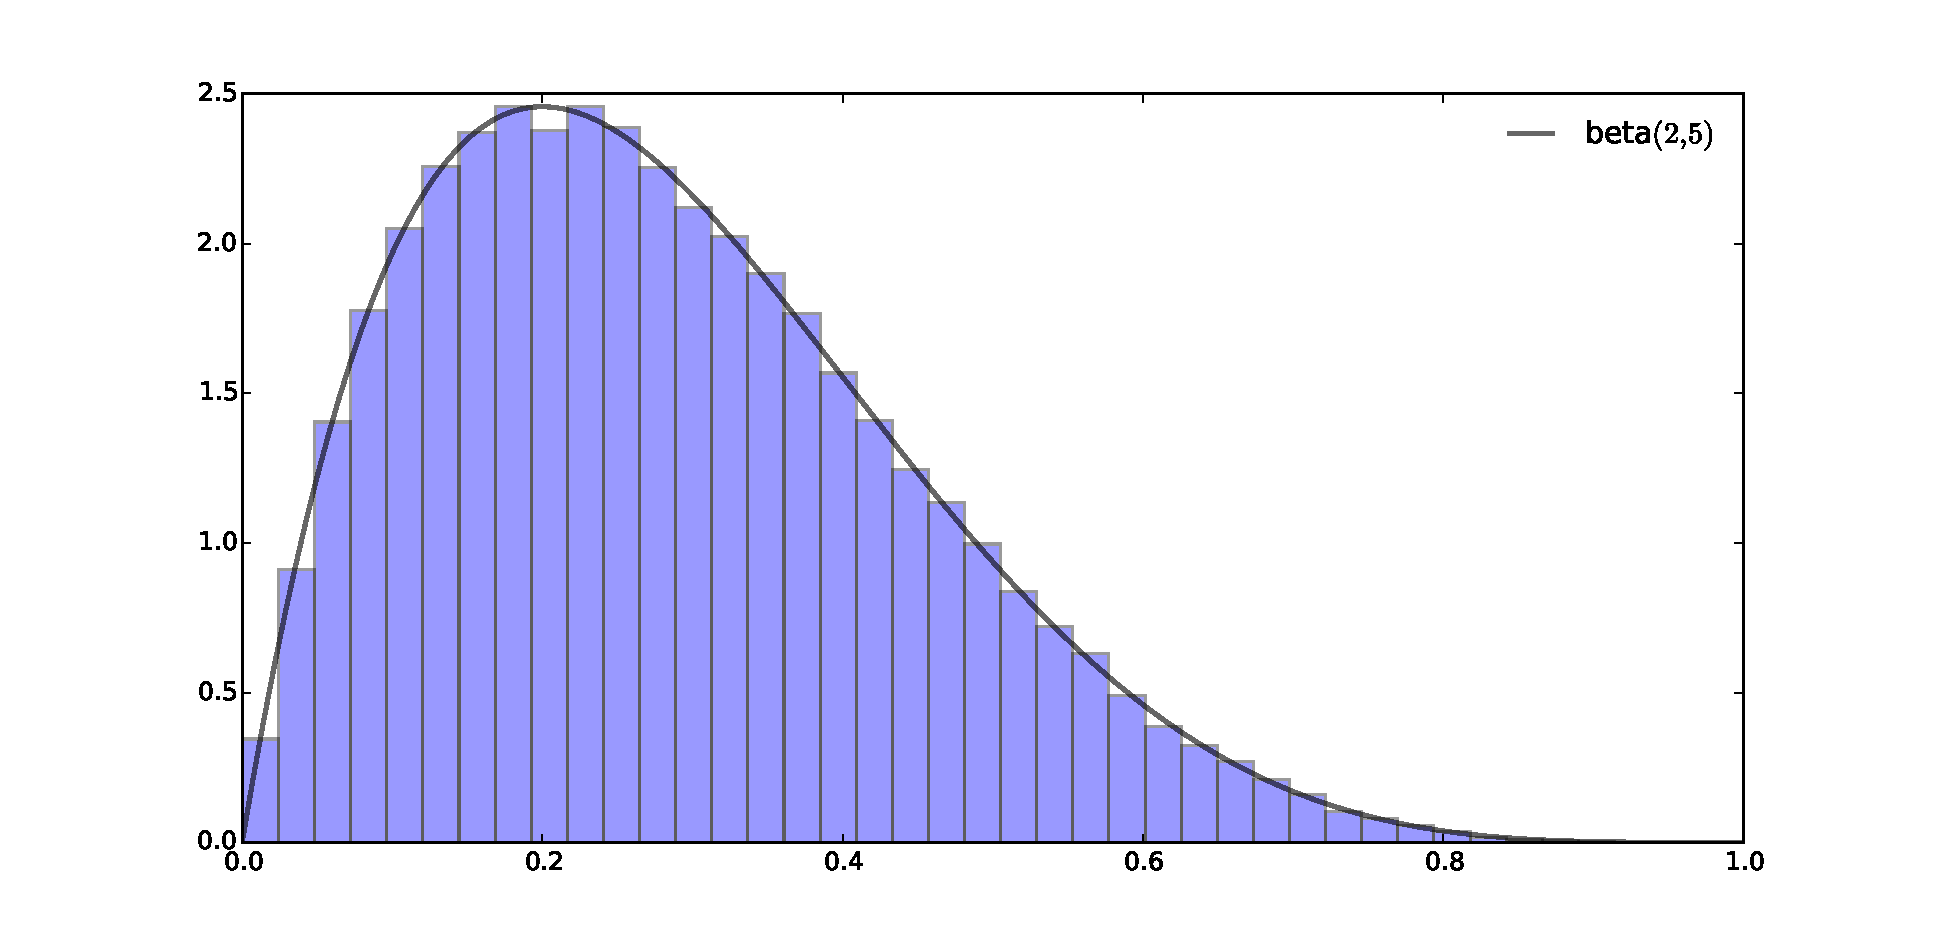
\includegraphics[trim={0 0em 0 2em}, clip]{rw_metropolis.pdf}}
        \caption{\label{f:rw_metropolis} Observations from the random walk Metropolis--Hastings
        algorithm when $\pi$ is the beta distribution}
    \end{figure}

\end{frame}


\end{document}
